

%%%%%%%%%%%%%%%%%%%%%%%%%%%%%%%%%%%

\begin{frame}
\frametitle{Filtros de fase mínima/máxima }

\vspace{-0.2cm}



\begin{itemize}
\footnotesize
\item Esta clasificación se basa en la posición de los ceros de un sistema.

\visible<2->{

\item \color{olivegreen}Ejemplo: dos sistemas con el mismo polo y ceros invertidos



\begin{itemize}

\color{gray}
\footnotesize

\item $H_1(z)=\frac{z+b}{z+a}$   con $|a|<1$ y $|b|<1$  $\rightarrow Z_{POLO}=-a$ y  $Z_{CERO}=-b$






\item $H_2(z)=\frac{bz+1}{z+a}$   con $|a|<1$ y $|b|<1$ $\rightarrow Z_{POLO}=-a$ y  $Z_{CERO}=-1/b$


\vspace{0.1cm}

$H_2(z)=\frac{bz+1}{z+a}\frac{z+b}{z+b}=\frac{z+b}{z+a}\frac{bz+1}{z+b}=H_1(z)H_{PasoToda}(z)$

\vspace{0.1cm}

$H_2(e^{jw})=H_1(e^{jw})H_{PT}(e^{jw})$ 

\vspace{0.1cm}

\scriptsize

\hspace{1cm}$\rightarrow |H_2(e^{jw})|=|H_1(e^{jw})||H_{PT}(e^{jw})|=|H_1(e^{jw})|$

\vspace{0.1cm}

\hspace{1cm}$\rightarrow arg(H_2(e^{jw}))=arg(H_1(e^{jw}))+arg(H_{PT}(e^{jw}))=$

\vspace{0.1cm}

\hspace{3.1cm}$=arg(H_1(e^{jw}))-\alpha(w)$ con $0<\alpha(w)<\pi$



\color{black}

\end{itemize}

}

\vspace{-0.3cm}

\visible<3->{

\color{black}

\item Generalización:

\begin{itemize}
\footnotesize
\item $H_{MIN}(z)$: FT causal estable con todos sus ceros dentro del círculo unidad

\item $H_{MAX}(z)$: FT causal estable con todos sus ceros simétricos respecto al círculo unidad y el caso anterior

\item $H_{MAX}(z)=H_{MIN}(z)H_{PasoToda}(z)$ con $H_{PT}(z)$ filtro paso todo estable en base a los ceros de $H_{MIN}(z)$

\item $|H_{MAX}(e^{jw})|=|H_{MIN}(e^{jw})|$


\item $arg(H_{MAX}(e^{jw}))=arg(H_{MIN}(e^{jw}))-\alpha(w)$ con $0<\alpha(w)<N\pi$ y N el número de ceros del filtro.


\end{itemize}


}


\end{itemize}
\end{frame}


\begin{frame}
\frametitle{Ejemplo Filtro Fase  Mínima y Máxima}
\footnotesize

\color{olivegreen} Dado un filtro con polos en 0.5, 0.1+0.3j y 0.1-0.3j, y los ceros en 0.3j, -0.3j y 4, determinar el comportamiento del desfase introducido por el filtro. Determinar los filtros de fase mínima y fase máxima asociados con el filtro.

\vspace{-0.4cm}

\color{gray}

\begin{columns}[c]
\begin{column}{5cm}
\lstinputlisting{./Matlab/EjFaseMinima.m}
\end{column}
\begin{column}{5cm}
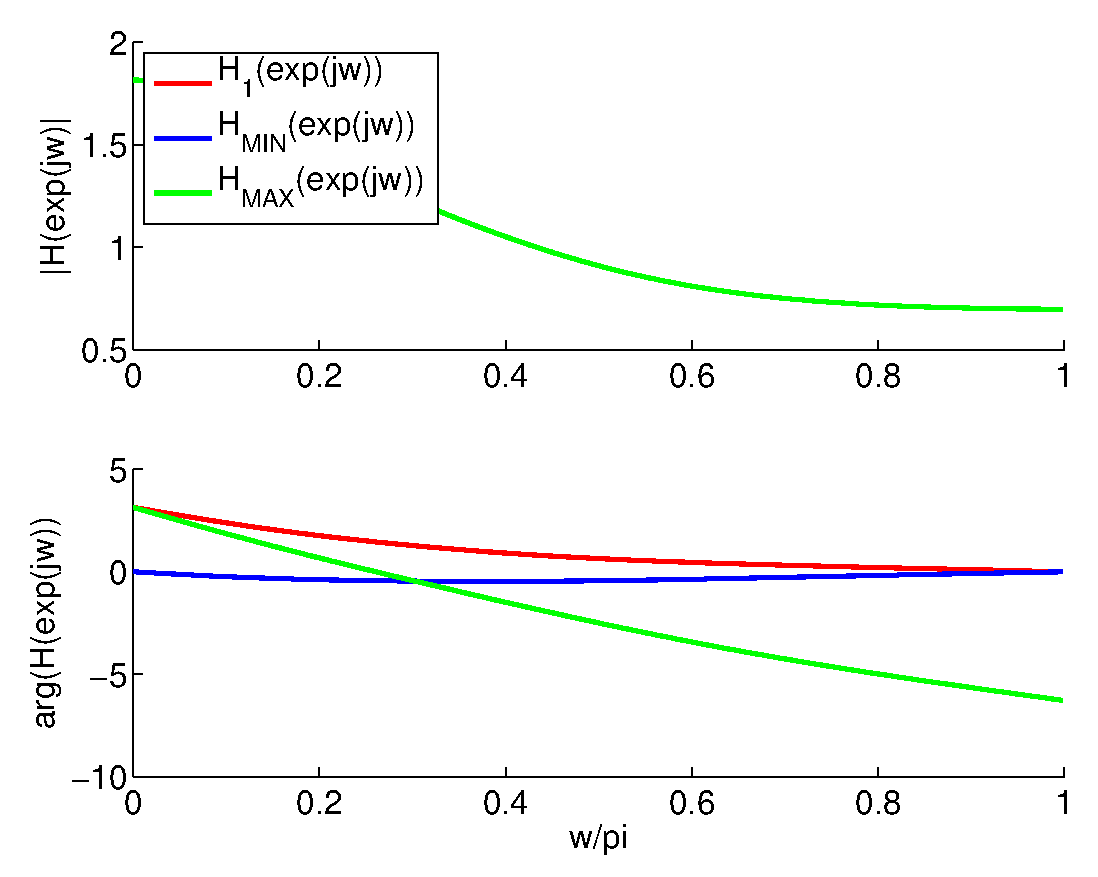
\includegraphics[width=5cm]{./Figures/EjFaseMinima.eps}
\end{column}
\end{columns}

\end{frame}
